\pdfoutput=1
\documentclass[a4paper,pdflatex,ja=standard]{bxjsarticle}

% ---Setting about the geometry of the document----
% \usepackage{a4wide}
% \pagestyle{empty}

% ---Physics and Math Packages---
\usepackage{amssymb,amsfonts,amsthm,mathtools}
\usepackage{physics,braket,bm}

% ---underline---
\usepackage{ulem}

% --- sorround the texts or equations
% \usepackage{fancybox,ascmac}

% ---settings of theorem environment---
% \usepackage{amsthm}
% \theoremstyle{definition}

% ---settings of proof environment---
% \renewcommand{\proofname}{\textbf{証明}}
% \renewcommand{\qedsymbol}{$\blacksquare$}

% ---Ignore the Warnings---
\usepackage{silence}
\WarningFilter{latexfont}{Some font shapes,Font shape}

% ---Insert the figure (If insert the `draft' at the option, the process becomes faster)---
\usepackage{graphicx}
% \usepackage{subcaption}

% ----Add a link to a text---
\usepackage{url}
\usepackage{xcolor,hyperref}
\hypersetup{colorlinks=true,citecolor=orange,linkcolor=blue,urlcolor=magenta}
\usepackage{bxcjkjatype}

% ---Tikz---
\usepackage{tikz,pgf,pgfplots,circuitikz}
\pgfplotsset{compat=1.15}
\usetikzlibrary{intersections,arrows.meta,angles,calc,3d,decorations.pathmorphing}

% ---Add the section number to the equation, figure, and table number---
\makeatletter
   \renewcommand{\theequation}{\thesubsection.\arabic{equation}}
   \@addtoreset{equation}{section}
   
   \renewcommand{\thefigure}{\thesection.\arabic{figure}}
   \@addtoreset{figure}{section}
   
   \renewcommand{\thetable}{\thesection.\arabic{table}}
   \@addtoreset{table}{section}
\makeatother

% ---enumerate---
\renewcommand{\labelenumi}{\arabic{enumi}.}
\renewcommand{\labelenumii}{(\roman{enumii})}

% ---Index---
% \usepackage{makeidx}
% \makeindex 

% ---Fonts---
\renewcommand{\familydefault}{\sfdefault}

% ---Title---
\title{東京大学\ 平成31年\ 物理学専攻\ 院試\ 解答例}
\author{ミヤネ}
\date{最終更新:\today}

\newcommand{\prb}[2]{
  \phantomsection
  \addcontentsline{toc}{subsection}{問題 #1: #2}
  \subsection*{第#1問}
  \setcounter{subsection}{#1}
  \setcounter{equation}{0}
}

\begin{document}

\maketitle

\tableofcontents
\clearpage

\section{数学パート}

\prb{1}{線形代数}
\begin{enumerate}
  \item 
  \begin{enumerate}
    \item 
    
    \uline{エルミートであること}

    エルミート共役をとれば
    \begin{align}
      (i[A,B])^{\dagger}
      &=
      -i(AB-BA)^{\dagger}
      \nonumber
      \\
      &=
      -i(B^{\dagger}A^{\dagger}-A^{\dagger}B^{\dagger})
      \nonumber
      \\
      &=
      i(AB-BA)
    \end{align}
    なので,エルミート性が示された\footnote{ここで,$(AB)^{\dagger}=B^{\dagger}A^{\dagger}$を用いています.}.

    \uline{トレースレスであること}

    行列$AB$の対角成分は
    \begin{equation}
      \tr AB
      =
      \sum_{i,j}a_{ij}b_{ji}
      =
      \tr BA
    \end{equation}
    なので,$\tr [A,B]=0$である.

    \item 

    $UU^{\dagger}$を計算すれば
    \begin{equation}
      UU^{\dagger}
      =
      \sum_{k=0}^{\infty}\frac{(iA)^{k}}{k!}
      \sum_{l=0}^{\infty}\frac{(-iA)^{l}}{l!}
      =
      \sum_{n=0}^{\infty}
      \frac{(iA)^{n}}{n!}
      \sum_{k=0}^{n}
      \binom{n}{k}(-1)^{n-k}
      =
      1
      +
      \sum_{n=1}^{\infty}
      \frac{(iA)^{n}}{n!}
      \cdot(1-1)^{n}
      =
      1
    \end{equation}
    である\footnote{これと同じノリで
    \begin{equation}
      e^{A}e^{B}
      =
      e^{A+B}
    \end{equation}
    を示せるはずです.}.なお,$n=k+l$で足し合わせ,$n=0$は別で計算して$n\geq 1$は二項定理を用いた.

    \item 

    計算すれば
    \begin{equation}
      \det U
      =
      \det 1
      +
      \sum_{n=1}^{\infty}\frac{(\det A)^{n}}{n!}
      =
      1
    \end{equation}
    である.

  \end{enumerate}

  \item 

  それぞれ
  \begin{equation}
    T_{1}
    =
    \begin{pmatrix}
      0 & 1 & 0 \\
      1 & 0 & 0 \\
      0 & 0 & 0
    \end{pmatrix}
    \ ,\ \ 
    T_{2}
    =
    \begin{pmatrix}
      0 & -i & 0 \\
      i & 0 & 0 \\
      0 & 0 & 0
    \end{pmatrix}
    \ ,\ \ 
    T_{7}
    =
    \begin{pmatrix}
      1 & 0 & 0 \\
      0 & 0 & 0 \\
      0 & 0 & -1
    \end{pmatrix}
  \end{equation}
  である.

  \item 

  $[T_{7},T_{1}]$は
  \begin{align}
    [T_{7},T_{1}]
    &=
    T_{7}T_{1}-T_{1}T_{7}
    \nonumber
    \\
    &=
    \begin{pmatrix}
      0 & 1 & 0 \\
      0 & 0 & 0 \\
      0 & 0 & 0
    \end{pmatrix}
    -
    \begin{pmatrix}
      0 & 0 & 0 \\
      1 & 0 & 0 \\
      0 & 0 & 0
    \end{pmatrix}
    \nonumber
    \\
    &=
    \begin{pmatrix}
      0 & 1 & 0 \\
      -1 & 0 & 0 \\
      0 & 0 & 0
    \end{pmatrix}
    \nonumber
    \\
    &=
    iT_{2}
  \end{align}
  なので,$A_{71,2}=1$である.

  同様に
  \begin{equation}
    T_{5}
    =
    \begin{pmatrix}
      0 & 0 & 0 \\
      0 & 0 & 1 \\
      0 & 1 & 0
    \end{pmatrix}
    \ ,\ \ 
    T_{6}
    =
    \begin{pmatrix}
      0 & 0 & 0 \\
      0 & 0 & -i \\
      0 & i & 0
    \end{pmatrix}
    \ ,\ \ 
    T_{8}
    =
    \begin{pmatrix}
      0 & 0 & 0 \\
      0 & 1 & 0 \\
      0 & 0 & -1
    \end{pmatrix}
  \end{equation}
  なので
  \begin{equation}
    [T_{5},T_{6}]
    =
    2i
    \begin{pmatrix}
      0 & 0 & 0 \\
      0 & 1 & 0 \\
      0 & 0 & -1
    \end{pmatrix}
    =
    2iT_{8}
  \end{equation}
  より$A_{56,8}=2$である.

  \item 

  \begin{enumerate}
    \item 

    $T$はエルミートなので
    \begin{align}
      G_{a}^{\prime}
      &=
      x^{\dagger}U^{\dagger}T_{a}Uy
      \nonumber
      \\
      &=
      x^{\dagger}e^{-i\theta T}T_{a}e^{i\theta T}y
      \nonumber
      \\
      &=
      x^{\dagger}
      \left( 1 - i\theta T +\mathcal{O}(\theta^2) \right)
      T_{a}
      \left( 1 + i\theta T +\mathcal{O}(\theta^2) \right)
      y
      \nonumber
      \\
      &=
      x^{\dagger}T_{a}y
      +
      i\theta x^{\dagger}[T_{a},T]y
      +
      \mathcal{O}(\theta^2)
      \nonumber
      \\
      &=
      x^{\dagger}T_{a}y
      +
      i\theta\sum_{b=1}^{8}
      \left(  
        \sum_{c=1}^{8}i\alpha_{c}A_{ac,b}
      \right)
      G_{b}
      +
      \mathcal{O}(\theta^2)
    \end{align}
    なので,
    \begin{equation}
      H_{ab}
      =
      \sum_{c=1}^{8}i\alpha_{c}A_{ac,b}
    \end{equation}
    である.

    \item 

    $x^{\prime}_{j},y_{k}^{\prime}$を計算すると,
    \begin{equation}
      x^{\prime}_{j}
      =
      U_{ja}x_{a}
      =
      x_{j}+i\theta T_{ja}x_{a}+\mathcal{O}(\theta^2)
      \ ,\ \ 
      y_{k}^{\prime}
      =
      y_{k}+i\theta T_{kb}y_{b}+\mathcal{O}(\theta^2)
    \end{equation}
    なので
    \begin{align}
      z_{i}^{\prime}
      &=
      \varepsilon_{ijk}
      \left\{  
        x_{j}+i\theta T_{ja}x_{a}+\mathcal{O}(\theta^2)
      \right\}
      \left\{  
        y_{k}+i\theta T_{kb}y_{b}+\mathcal{O}(\theta^2)
      \right\}
      \nonumber
      \\
      &=
      z_{i}
      +
      i\theta\varepsilon_{ijk}
      \left\{  
        T_{ja}x_{a}y_{k}
        +
        T_{kb}x_{j}y_{b}
      \right\}
      +
      \mathcal{O}(\theta^2)
      \label{z_prime}
    \end{align}
    である.ここで
    \begin{equation}
      \varepsilon_{abi}z_{i}
      =
      \varepsilon_{abi}\varepsilon_{ijk}x_{j}y_{k}
      =
      x_{a}y_{b}-x_{b}y_{a}
    \end{equation}
    であり,
    \begin{align}
      \varepsilon_{ijk}
      \left\{  
        T_{ja}x_{a}y{k}
        +
        T_{kb}x_{j}y_{b}
      \right\}
      &=
      \varepsilon_{ijk}
      \left\{  
        T_{ja}x_{a}y_{k}
        -
        T_{ja}x_{k}y_{a}
      \right\}
      \nonumber
      \\
      &=
      \varepsilon_{ijk}T_{ja}
      \left[ x_{a}y_{k}-x_{k}y_{a} \right]
      =
      \varepsilon_{ijk}\varepsilon{kac}T_{ja}z_{c}
    \end{align}
    なので
    \begin{equation}
      i\theta\varepsilon_{ijk}
      \left\{  
        T_{ja}x_{a}y_{k}
        +
        T_{kb}x_{j}y_{b}
      \right\}
      =
      i\theta\varepsilon_{ijk}\varepsilon{kac}T_{ja}z_{c}
      \eqqcolon
      i\theta M_{ic}z_{c}
    \end{equation}
    より
    \begin{equation}
      M_{ij}
      =
      \varepsilon_{ilk}\varepsilon{kaj}T_{la}
      =
      T_{ji}-T_{ij}
    \end{equation}
    である\footnote{いろいろごちゃごちゃしてしまいました.もう少しスマートに答えられるはずです.}.
  \end{enumerate}
\end{enumerate}



\clearpage
\prb{2}{微積分}
\begin{enumerate}
  \item 
  微分方程式は
  \begin{equation}
    \dv[2]{f_{\alpha}^{(n)}}{x}
    =
    -(m_{\alpha}^{2}+\lambda_{\alpha}^{(n)})f_{\alpha}^{(n)}
  \end{equation}
  なので,$\omega_{\alpha}\coloneqq m_{\alpha}^{2}+\lambda_{\alpha}^{(n)}$とすれば,一般解は
  \begin{equation}
    f_{\alpha}^{(n)}(x)
    =
    Ae^{i\omega x}
    +
    Be^{-i\omega x}
  \end{equation}
  である.境界条件は
  \begin{equation}
    \cos \omega_{\alpha}\pi=0
    \ ,\ \ 
    A=B
  \end{equation}
  であり,規格化はしないので$A=1$とすれば
  \begin{equation}
    \omega_{\alpha}
    =
    n+\frac{1}{2}
  \end{equation}
  であり,固有値は
  \begin{equation}
    \lambda_{\alpha}^{(n)}
    =
    -m_{\alpha}^{2}
    +
    \left( n+\frac{1}{2} \right)^{2}
  \end{equation}
  であり,固有関数は
  \begin{equation}
    f_{\alpha}^{(n)}(x)
    =
    2\cos\left( n+\frac{1}{2} \right)x
  \end{equation}
  である.

  \item 
  \begin{enumerate}
    \item 
    $\log(\lambda^{-s})=-s\log\lambda$の両辺を$s$で微分して整理すれば
    \begin{equation}
      (\lambda^{-s})'
      =
      -\lambda^{-s}\log\lambda
    \end{equation}
    である.

    \item 
    $Z'(0)$を計算すると
    \begin{equation}
      Z'(0)
      =
      \sum_{n=0}^{\infty}
      \left[  
        \log\frac{\lambda_{1}^{n}}{\lambda_{2}^{n}}
      \right]
      =
      \log\prod_{n=0}^{\infty}\frac{\lambda_{1}^{n}}{\lambda_{2}^{n}}
    \end{equation}
    なので
    \begin{equation}
      D=e^{-Z'(0)}
      \label{D}
    \end{equation}
    である.

    \item
    微分方程式の解は,1.と同様にして
    \begin{equation}
      g_{\alpha}(x;\lambda)
      =
      Ae^{i\omega x}
      +
      Be^{-i\omega x}
    \end{equation}
    なので,これに初期条件を代入すれば
    \begin{equation}
      A+B=1
      \ ,\ \ 
      A=B
    \end{equation}
    となるので,求める解は
    \begin{equation}
      g_{\alpha}(x;\lambda)
      =
      \cos\omega x
      \ ,\ \ 
      \omega
      \coloneqq
      \sqrt{m_{\alpha}^2+\lambda}
    \end{equation}
    である.

    \item 
    $\tilde{g}_{\alpha}^{\prime}/\tilde{g}_{\alpha}$は,
    \begin{align}
      \frac{1}{\tilde{g}_{\alpha}(\lambda)}\dv{\tilde{g}_{\alpha}(\lambda)}{\lambda}
      &=
      \frac{1}{k_{\alpha}^{(n)}(\lambda-\lambda_{\alpha}^{(n)})+\mathcal{O}[(\lambda-\lambda_{\alpha}^{n})^2]}
      \cdot
      \left( k_{\alpha}^{(n)}+\mathcal{O}[(\lambda-\lambda_{\alpha}^{n})] \right)
      \nonumber
      \\
      &=
      \frac{1+\mathcal{O}[\lambda-\lambda_{\alpha}^{n}]}{\lambda-\lambda_{\alpha}^{(n)}+\mathcal{O}[(\lambda-\lambda_{\alpha}^{n})^2]}
      =
      \frac{1}{\lambda-\lambda_{\alpha}^{(n)}}
    \end{align}
    である.したがって,留数定理より
    \begin{equation}
      \int_{C}\lambda^{-s}\left[  
        \frac{1}{\lambda-\lambda_{2}^{n}}
        -
        \frac{1}{\lambda-\lambda_{1}^{n}}
      \right]
      \dd \lambda
      =
      2\pi i\sum_{n=0}^{\infty}\left[ \left( \lambda_{2}^{(n)} \right)^{-s} - \left( \lambda_{1}^{(n)} \right)^{-s} \right]
      =
      2\pi i Z(s)
    \end{equation}
    である.よって,$A=1/2\pi i$であり,
    \begin{equation}
      Z(s)
      =
      \frac{1}{2\pi i}
      \int_{C}\lambda^{-s}
      \left[  
        \frac{1}{\tilde{g}_{2}(\lambda)}\dv{\tilde{g}_{2}(\lambda)}{\lambda}
        -
        \frac{1}{\tilde{g}_{1}(\lambda)}\dv{\tilde{g}_{1}(\lambda)}{\lambda}
      \right]
      \dd \lambda
      \label{sol4}
    \end{equation}
    である.

    \item 
    \eqref{sol4}より,$Z'(0)$は
    \begin{equation}
      Z'(0)
      =
      -\frac{1}{2\pi i}
      \int_{C}
      \log \lambda
      \left[  
        \frac{1}{\tilde{g}_{2}(\lambda)}\dv{\tilde{g}_{2}(\lambda)}{\lambda}
        -
        \frac{1}{\tilde{g}_{1}(\lambda)}\dv{\tilde{g}_{1}(\lambda)}{\lambda}
      \right]
      \dd \lambda
    \end{equation}
    である\footnote{もちろん,この式変形が許されているかどうかはわかりませんが,少なくとも経路上では解析的なのでいいんじゃないかと思います.}.この経路で計算するとき,$C_{\text{in}}$のときの$\lambda$の偏角が$\theta$で,$C_{\text{out}}$のときの$\lambda$の偏角が$\theta-2\pi$であることに気をつければ
    \begin{align}
      &\hspace{1cm}
      \int_{C}
      \log \lambda
      \left[  
        \frac{1}{\tilde{g}_{2}(\lambda)}\dv{\tilde{g}_{2}(\lambda)}{\lambda}
        -
        \frac{1}{\tilde{g}_{1}(\lambda)}\dv{\tilde{g}_{1}(\lambda)}{\lambda}
      \right]
      \dd \lambda
      \nonumber
      \\
      &=
      \int_{C_{\text{in}}}+\int_{C_{\text{out}}}
      \nonumber
      \\
      &=
      \int_{\infty}^{0}
      \log (Re^{i\theta})
      \left[  
        \vphantom{\frac{1}{\tilde{g}_{2}(\lambda)}\dv{\tilde{g}_{2}(\lambda)}{\lambda}
        -
        \frac{1}{\tilde{g}_{1}(\lambda)}\dv{\tilde{g}_{1}(\lambda)}{\lambda}}
        \cdots\cdots
      \right]
      \dd (Re^{i\theta})
      +
      \int_{0}^{\infty}
      \log (Re^{i(\theta-2\pi)})
      \left[  
        \vphantom{\frac{1}{\tilde{g}_{2}(\lambda)}\dv{\tilde{g}_{2}(\lambda)}{\lambda}
        -
        \frac{1}{\tilde{g}_{1}(\lambda)}\dv{\tilde{g}_{1}(\lambda)}{\lambda}}
        \cdots\cdots
      \right]
      \dd (Re^{i(\theta-2\pi)})
      \nonumber
      \\
      &=
      2\pi i
      \int_{C_{\text{in}}}
      \left[  
        \frac{1}{\tilde{g}_{2}}\dv{\tilde{g}_{2}(\lambda)}{\lambda}
        -
        \frac{1}{\tilde{g}_{1}}\dv{\tilde{g}_{1}(\lambda)}{\lambda}
      \right]
      \dd \lambda
    \end{align}
    となる\footnote{もう少し丁寧に言うと,$\log(Re^{i(\theta-2\pi)})=\log (Re^{i\theta})-2\pi i$です.}.この積分はもはや極などとは関係なく$\lambda$を$0\rightarrow\infty\cdot e^{i\theta}$で積分してよいので,
    \begin{align}
      &\int_{0}^{\infty\cdot e^{i\theta}}
      \left[  
        \dv{}{\lambda}\left[ \log \tilde{g}_{2}(\lambda) \right]
        -
        \dv{}{\lambda}\left[ \log \tilde{g}_{1}(\lambda) \right]
      \right]
      \dd \lambda
      \nonumber
      \\
      &\hspace{3cm}
      =
      \log \tilde{g}_{2}(\infty\cdot e^{i\theta})
      -
      \log \tilde{g}_{2}(0)
      -
      \log \tilde{g}_{1}(\infty\cdot e^{i\theta})
      +
      \log \tilde{g}_{1}(0)
    \end{align}
    である.ここで,
    \begin{equation}
      \tilde{g}_{\alpha}(\infty\cdot e^{i\theta})
      =
      \cos(\pi\sqrt{m_{\alpha}^2+\infty\cdot e^{i\theta}})
      \sim
      \cos\left( \pi\sqrt{\infty\cdot e^{i\theta}}  \right)
      \label{g_alpha}
    \end{equation}
    なので,$\tilde{g}_{\alpha}(\infty\cdot e^{i\theta})$の引き算は消去できて
    \begin{equation}
      Z'(0)
      \sim
      \log \frac{\tilde{g}_{2}}{\tilde{g}_{1}}
    \end{equation}
    である.

    \item 
    具体的に計算すると
    \begin{equation}
      Z'(0)
      =
      \log
      \frac{\cos \pi m_{2}}{\cos \pi m_{1}}
    \end{equation}
    なので,\eqref{D}に代入すれば
    \begin{equation}
      D
      =
      \frac{\cos \pi m_{1}}{\cos \pi m_{2}}
    \end{equation}
    である\footnote{$m_{\alpha}<1/2$なのは,$\log$の中に$\cos$が入ってくるからです.}.
    
  \end{enumerate}
\end{enumerate}

\subsection*{補足}

\begin{itemize}
  \item 
  ブランチカットを気にするべき例題は
  \begin{equation}
    I
    =
    \int_{0}^{\infty}
    \frac{\log x}{(1+x)^3}\dd x
    \label{int_exm}
  \end{equation}
  とかでしょうか.これは図\ref{cont}のような経路をとりますが,$\Gamma_{2}$のところの積分で少し注意が必要です.

  \begin{figure}[ht]
    \centering    
    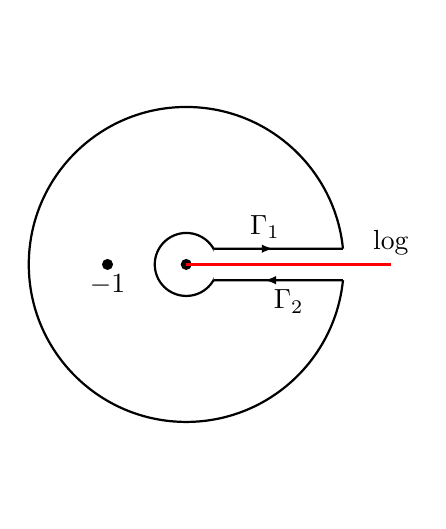
\begin{tikzpicture}[scale=1] 
        \draw[thick, name path=C1] (0,0) circle (2);       
        \draw[thick, name path=C2] (0,0) circle (0.4);
        \fill[black] (0,0) circle (2pt);
        \draw [opacity=0.0, name path=line1] (0,0.2)--(2.1,0.2);       
        \draw [opacity=0.0] (0,-3)--(0,3);        
        \draw [opacity=0.0, name path=line2] (0,-0.2)--(2.1,-0.2);
        \draw [name intersections={of= C1 and line1, by={a}}];
        \draw [name intersections={of= C2 and line1, by={b}}];        
        \draw [name intersections={of= C1 and line2, by={c}}];
        \draw [name intersections={of= C2 and line2, by={d}}];
        \fill [white] (d)--(2.1,-0.2)--(2.1,0.2)--(b)--cycle;
        \draw[thick] (d)--(c);
        \draw[thick] (b)--(a);
        \draw (1.0,0.2) node[above]{$\Gamma_{1}$};        
        \draw (1.3,-0.2) node[below]{$\Gamma_{2}$};
        \fill (-1,0) circle (2pt) node[below] {$-1$};
        \draw [-latex, thin] (b)--(1.1,0.2);
        \draw [-latex, thin] (c)--(1.0,-0.2);
        \draw [red, thick] (0,0)--(2.6,0);
        \draw (2.6,0) node [above]{$\log$};
      \end{tikzpicture}    
      \caption{積分路}
      \label{cont}
  \end{figure}

  この積分\eqref{int_exm}をもとめるためには,すこしテクニカルではありますが
  \begin{equation}
    f(z)
    =
    \frac{(\log z)^2}{(1+z)^3}
  \end{equation}
  を図\ref{cont}で積分します.経路のうち,外側の経路の寄与は無視できるので
  \begin{equation}
    \int_{\Gamma_{1}}f
    +
    \int_{\Gamma_{2}}f
    =
    2\pi i\Res[f,-1]
    \label{int_all}
  \end{equation}
  です.$z=-1$が3位の極であることから,$n$位の極に対する公式
  \begin{equation}
    \Res[f,a]
    =
    \frac{1}{(n-1)!}
    \lim_{z\rightarrow a}
    \dv[n-1]{}{z}
    \left[ (z-a)^{n}f(z) \right]
  \end{equation}
  を用いれば\footnote{この公式の証明は案外簡単で,$f(z)$のローラン展開
  \begin{equation}
    \nonumber
    f(z)
    =
    \frac{a_{-n}}{(z-a)^{n}}
    +
    \frac{a_{-n+1}}{(z-a)^{n-1}}
    +
    \cdots
    +
    \frac{a_{-1}}{z-a}
    +
    a_{0}
    +
    a_{1}(z-a)
    +
    \cdots
  \end{equation}
  のなかから$a_{-1}$だけを取り出すために$(z-a)^{n}f(z)$を計算して,$n-1$階だけ微分してやります.あとは,
  \begin{equation}
    \nonumber
    \oint_{\gamma}\frac{\dd z}{z-a}
    =
    2\pi i
  \end{equation}
  とするだけです.
  },
  \begin{equation}
    2\pi i\Res[f,-1]
    =
    2\pi i
    \cdot
    \frac{1}{2}\lim_{z\rightarrow -1}
    \dv[2]{}{z}\left[ (\log z)^2 \right]
    =
    2\pi i(1-i\pi)
  \end{equation}
  です.さて,経路の部分ですが,$\Gamma_{1}$の部分は普通に
  \begin{equation}
    \int_{\Gamma_{1}}f
    =
    \int_{0}^{\infty}\frac{(\log x)^2}{(1+x)^3}\dd x
  \end{equation}
  でよいです.問題は$\Gamma_{2}$での積分なのですが,ここで積分するときは,$z$の偏角は$2\pi i$であることに注意しなくてはなりません\footnote{
    もちろん大丈夫だと思いますが,
    \begin{equation}
      \log z
      =
      \log |z|
      +
      i\arg z
      \nonumber
    \end{equation}
    です.実は先ほどの留数の計算でもこっそりと用いてました.
  }.つまり
  \begin{equation}
    \int_{\Gamma_{2}}f
    =
    \int_{\infty}^{0}\frac{(\log x+2\pi i)^2}{(1+x)^3}\dd x
    =
    -\int_{0}^{\infty}\frac{(\log x)^2+4\pi i\log x-4\pi^2}{(1+x)^3}\dd x
  \end{equation}
  となっています.あとは,\eqref{int_all}を計算するだけで
  \begin{equation}
    I
    =
    \int_{0}^{\infty}
    \frac{\log x}{(1+x)^3}\dd x
    =
    -\frac{1}{2}
  \end{equation}
  ともとまります.少し$f(z)$を不気味な形にしてやりましたが,あれでうまくいきました.  

  \item 
  \eqref{g_alpha}の引き算が$0$とできることですが,ちゃんとやるためには
  \begin{equation}
    \tilde{g}_{\alpha}(\lambda)
    =
    \frac{e^{i\pi\sqrt{m_{\alpha}^2+\lambda}}+e^{-i\pi\sqrt{m_{\alpha}^2+\lambda}}}{2}
  \end{equation}
  として,うまくいくことを言わなくてはなりません.第1項は
  \begin{align*}
    e^{i\pi\sqrt{m_{\alpha}^2+\lambda}}
    &=
    \exp\left[  
      i\pi \exp\left[ \frac{1}{2}\log (m_{\alpha}^2+\lambda) \right]
    \right]
    \nonumber
    \\
    &=
    \exp\left[  
      i\pi \exp\left[ 
        \frac{1}{2}(\log |m_{\alpha}^2+\lambda|+i\pi\arg(m_{\alpha}^2+\lambda)) \right]
    \right]
    \nonumber
    \\
    &=
    \exp\left[  
      i\pi e^{\log\sqrt{|m_{\alpha}^2+\lambda|}}(\cos(\pi\arg(m_{\alpha}^2+\lambda)/2)+i\sin(\pi\arg(m_{\alpha}^2+\lambda)/2))
    \right]
    \nonumber
    \\
    &=
    e^{-\pi \sqrt{|m_{\alpha}^2+\lambda|}\sin(\pi\arg(m_{\alpha}^2+\lambda)/2)}\cdot e^{i\cdots}
  \end{align*}
  ですが,$\lambda\rightarrow\infty\cdot e^{i\theta}$のときは.ちゃんと$\sqrt{|m_{\alpha}^2+\lambda|}\sin(\pi\arg(m_{\alpha}^2+\lambda)/2)\rightarrow\infty$なので,この項は$0$に行ってくれます.よって,第2項の引き算を考えればよくて,
  \begin{align*}
    &\hspace{1cm}
    |
    e^{-i\pi\sqrt{m_{2}^2+\lambda}}
    -
    e^{-i\pi\sqrt{m_{1}^2+\lambda}}
    |^2
    \nonumber
    \\
    &=
    |
    e^{\pi \sqrt{|m_{2}^2+\lambda|}\sin(\pi\arg(m_{2}^2+\lambda)/2)}\cdot e^{i\pi\log\sqrt{|m_{2}^2+\lambda|}\cos(\pi\arg(m_{2}^2+\lambda)/2)}
    \nonumber
    \\
    &\hspace{1cm}
    -
    e^{\pi \sqrt{|m_{1}^2+\lambda|}\sin(\pi\arg(m_{1}^2+\lambda)/2)}\cdot e^{i\pi\log\sqrt{|m_{1}^2+\lambda|}\cos(\pi\arg(m_{1}^{2}+\lambda)/2)}
    |^2
  \end{align*}
  ですが,これを実部虚部に分けると
  \begin{align}
    &\hspace{1cm}
    |
    e^{\pi \sqrt{|m_{2}^2+\lambda|}\sin(\pi\arg(m_{2}^2+\lambda)/2)}\cdot e^{i\pi\log\sqrt{|m_{2}^2+\lambda|}\cos(\pi\arg(m_{2}^2+\lambda)/2)}
    \nonumber
    \\
    &\hspace{2cm}
    -
    e^{\pi \sqrt{|m_{1}^2+\lambda|}\sin(\pi\arg(m_{1}^2+\lambda)/2)}\cdot e^{i\pi\log\sqrt{|m_{1}^2+\lambda|}\cos(\pi\arg(m_{1}^{2}+\lambda)/2)}
    |^2
    \nonumber
    \\
    &=
    \left(  
      e^{\pi \sqrt{|m_{2}^2+\lambda|}\sin(\pi\arg(m_{2}^2+\lambda)/2)}
      \cos(\pi\log\sqrt{|m_{1}^2+\lambda|}\cos(\pi\arg(m_{1}^{2}+\lambda)/2))
    \right.
      \nonumber
      \\
      &\hspace{1cm}\left.
      -
      e^{\pi \sqrt{|m_{1}^2+\lambda|}\sin(\pi\arg(m_{1}^2+\lambda)/2)}
      \cos(\pi\log\sqrt{|m_{2}^2+\lambda|}\cos(\pi\arg(m_{2}^2+\lambda)/2))
    \right)^2
    \nonumber
    \\
    &\hspace{1cm}
    +
    \left(  
      e^{\pi \sqrt{|m_{2}^2+\lambda|}\sin(\pi\arg(m_{2}^2+\lambda)/2)}
      \sin(\pi\log\sqrt{|m_{1}^2+\lambda|}\cos(\pi\arg(m_{1}^{2}+\lambda)/2))
    \right.
      \nonumber
      \\
      &\hspace{2cm}\left.
      -
      e^{\pi \sqrt{|m_{1}^2+\lambda|}\sin(\pi\arg(m_{1}^2+\lambda)/2)}
      \sin(\pi\log\sqrt{|m_{2}^2+\lambda|}\cos(\pi\arg(m_{2}^2+\lambda)/2))
    \right)^2
  \end{align}
  であり,これらの項がそれぞれ$0$に収束することを確認すればよいです.$\lambda\rightarrow\infty\cdot e^{i\theta}$のとき,$\arg$は$\theta$に漸近することが,福素平面での考察からわかり,また,$\sqrt{|m_{1}^2+\lambda|}$と$\sqrt{|m_{2}^2+\lambda|}$は同じ速度で発散するので,この考察から,それぞれの項が0になります\footnote{それぞれの項が収束するのもちゃんと示したいですが,ちょっと無理でした.}.よって,
  \begin{equation}
    \tilde{g}_{2}(\lambda)
    -
    \tilde{g}_{1}(\lambda)
    \rightarrow
    0
    \ \ \ 
    (\lambda\rightarrow\infty\cdot e^{i\theta})
  \end{equation}
  です\footnote{さすがに試験中はここまでする必要はないと思いますが.}.

\end{itemize}



\clearpage
\section{物理パート}
\prb{1}{量子力学}
\begin{enumerate}
  \item 
  計算すれば
  \begin{align}
    \left[ a,a^{\dagger} \right]
    &=
    1
    \\
    \left[ N,a \right]
    &=
    -a
    \\
    \left[ N,a^{\dagger} \right]
    &=
    a^{\dagger}
  \end{align}
  である.また,$\alpha=1,\beta=1/2$である.

  \item   
  $N$の固有状態と固有値をそれぞれ$\ket{\lambda},\lambda$としておく.非負であることは,
  \begin{equation}
    \|a\ket{\lambda}\|^2=\ev{\lambda|N|\lambda}=\lambda\geq 0
  \end{equation}
  からわかる.また,$a$が
  \begin{equation}
    a\ket{\lambda}
    \propto
    \ket{\lambda-1}
  \end{equation}
  であることから,
  \begin{equation}
    N\ket{\lambda}
    =
    0
  \end{equation}
  という固有値$0$の状態が存在しないと固有値が負になることが許されてしまうため,固有値が$0$の状態$\ket{0}$が存在し,固有値は整数になる.

  \item 
  エネルギーは
  \begin{equation}
    H\ket{n}
    =
    \frac{\hbar\omega}{2}\left( n+\frac{1}{2} \right)\ket{n}
  \end{equation}
  で,固有状態は
  \begin{equation}
    a\ket{n}
    =
    c\ket{n-1}
  \end{equation}
  とすれば
  \begin{equation}
    n
    =
    \ev{n|a^{\dagger}a|n}
    =
    |c|^2
  \end{equation}
  より,$c=1/\sqrt{n}$なので
  \begin{equation}
    \ket{n}
    =
    \frac{1}{\sqrt{n!}}(a^{\dagger})^{n}\ket{0}
  \end{equation}
  である.

  \item 
  \begin{enumerate}
    \item 
    $H$の固有状態が$\ket{\psi_{l}}$とすると
    \begin{equation}
      H\ket{\psi_{l}}
      =
      E_{\lambda}\ket{\psi_{l}}
      \label{eigen}
    \end{equation}
    であり,これらを展開すると
    \begin{equation}
      \begin{dcases}
        \ket{\psi_{l}}
        &=
        \ket{l}+\ket{l^{(1)}}+\ket{l^{(2)}}+\cdots
        \\
        E_{l}
        &=
        E_{l}^{(0)}
        +
        E_{l}^{(1)}
        +
        E_{l}^{(2)}
        +
        \cdots
      \end{dcases}
    \end{equation}
    であり,\eqref{eigen}に代入すれば
    \begin{equation}
      (H_{0}+V)
      (\ket{l}+\ket{l^{(1)}}+\ket{l^{(2)}}+\cdots)
      =
      (E_{l}^{(0)}
      +
      E_{l}^{(1)}
      +
      E_{l}^{(2)}
      +
      \cdots)
      (\ket{l}+\ket{l^{(1)}}+\ket{l^{(2)}}+\cdots)
    \end{equation}
    である.$H_{0}\ket{l}=E_{l}^{(0)}\ket{l}$に気をつければ,1次と2次の項は
    \begin{equation}
      \begin{dcases}
        1\text{次}
        &:
        V\ket{l}
        +
        H_{0}\ket{l^{(1)}}
        =
        E_{l}^{(0)}\ket{l^{(1)}}
        +
        E_{l}^{(1)}\ket{l}
        \\
        2\text{次}
        &:
        V\ket{l^{(1)}}
        +
        H_{0}\ket{l^{(2)}}
        =
        E_{l}^{(0)}\ket{l^{(2)}}
        +
        E_{l}^{(1)}\ket{l^{(1)}}
        +
        E_{l}^{(2)}\ket{l}
      \end{dcases}
      \label{pertur}
    \end{equation}
    である.第1式に$\bra{l}$をかければ
    \begin{equation}
      E_{n}^{(1)}
      =
      V_{nn}
    \end{equation}
    であり,\eqref{pertur}の第1式に$\bra{j}\ (j\neq l)$をかければ\footnote{ここで,$\ket{l}$と$\ket{l^{1}}$は直交しますが,$\ket{j}$と$\ket{l^{(1)}}$は必ずしも直交しないことに注意しましょう.}
    \begin{equation}
      \ev*{j|l^{(1)}}
      =
      \frac{V_{jl}}{E_{l}^{(0)}-E_{j}^{(0)}}
      \label{first}
    \end{equation}
    なので,\eqref{pertur}の第2式から
    \begin{equation}
      E_{l}^{(2)}
      =
      \sum_{k\neq l}
      \frac{|V_{kl}|^2}{E_{l}^{(0)}-E_{k}^{(0)}}
      \label{second}
    \end{equation}
    である.

    \item 
    $V_{k0}=\ev*{k|V|0}$なので,
    \begin{equation}
      x
      =
      \sqrt{\frac{\hbar}{2m\omega}}(a+a^{\dagger})
    \end{equation}
    に注意すれば
    \begin{equation}
      V_{k0}
      =
      \lambda\left( \frac{\hbar}{2m\omega} \right)^2
      \ev*{k|(a+a^{\dagger})^4|0}
      =
      \begin{dcases}
        2\cdot\lambda\left( \frac{\hbar}{2m\omega} \right)^2
        &(k=0)
        \\
        3\cdot\lambda\left( \frac{\hbar}{2m\omega} \right)^2
        &(k=2)
        \\
        \lambda\left( \frac{\hbar}{2m\omega} \right)^2
        &(k=4)
      \end{dcases}
    \end{equation}
    である\footnote{実際に計算すればわかりますが,$(a+a^{\dagger})^4$を展開したときに出てくるもので,許されるのは
    \begin{gather}
      aaa^{\dagger}a^{\dagger}
      \ ,\ \ 
      aa^{\dagger}aa^{\dagger}
      \ ,\ \ 
      aa^{\dagger}a^{\dagger}a^{\dagger}
      \ , 
      \nonumber\\
      a^{\dagger}aa^{\dagger}a^{\dagger}
      \ ,\ \ 
      a^{\dagger}a^{\dagger}aa^{\dagger}
      \ ,\ \ 
      a^{\dagger}a^{\dagger}a^{\dagger}a^{\dagger}
      \nonumber
    \end{gather}
    です.他のものは,$a\ket{0}=0$で消えてしまいます.}.よって,\eqref{first},\eqref{second}より
    \begin{align}
      E_{l}^{(1)}
      &=
      2\cdot\lambda\left( \frac{\hbar}{2m\omega} \right)^2
      \\
      E_{l}^{(2)}
      &=
      -\frac{19}{64}\cdot\frac{\lambda^2\hbar^3}{m^4\omega^5}
    \end{align}
    である\footnote{特に2次はおどろおどろしいですが,次元は
    \begin{equation}
      \frac{[M]^{2}[L]^{-4}[T]^{-4}\cdot[M]^{3}[L]^{6}[T]^{-3}}{[M]^{4}[T]^{-5}}
      =
      [M][L]^{2}[T]^{-2}
      \nonumber
    \end{equation}
    でちゃんとエネルギーです.($\lambda$の次元にはよく注意しましょう.)}.
  \end{enumerate}

  \item 
  次の等式
  \begin{equation}
    E_{n}
    =
    V(x)
  \end{equation}
  を満たす転回点を$x_{0},-x_{0}$とすると\footnote{今,準位が大きいところを考えているので,転回点は2つでしかも対称です.\label{comment}}
  \begin{equation}
    \int_{-x_{0}}^{x_{0}}\sqrt{E_{n}-\left(  
      \frac{m\omega^2}{2}x^2+\lambda x^4
    \right)}
    \dd x
    =\pi\hbar\left( n+\frac{1}{2} \right)
    \label{semiclas_cond}
  \end{equation}
  が量子化条件である.この積分は,図\ref{int_fig}の灰色の部分の面積に対応する\footnote{以後の議論はなかなか粗っぽいので,時間があれば数値計算できればと思っています.例えば,\eqref{semiclas_cond}は,$E_{n}$についての方程式になっていますが,$n$に対して両辺の値がうまく決まるような$E_{n}$を拾ってこなくてはなりません.}.

  \begin{figure}[ht]
    \centering    
    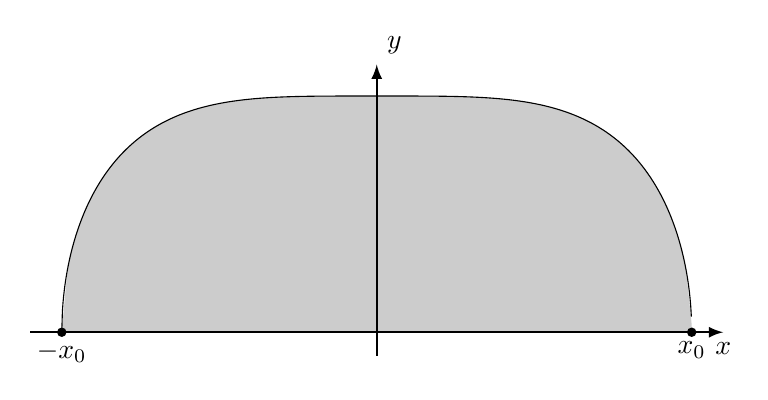
\begin{tikzpicture}[scale=1]       
      \fill[opacity=0.2] plot [smooth,samples=100,domain=-4:4] (\x,{sqrt(abs(4*4*4*4-\x*\x*\x*\x))/16*3}) -- (4,0) -- (-4,0);
      \draw[-latex,thick] (-4.4,0)--(4.4,0) node [below]{$x$};
      \draw[-latex,thick] (0,-0.3)--(0,3.4) node [above right] {$y$};
      \draw[name path=int, domain=-4:4,samples=1000] plot (\x,{sqrt(abs(4*4*4*4-\x*\x*\x*\x))/16*3});
      \fill(-4,0)circle(0.06)node[below]{$-x_0$};
      \fill(4,0)circle(0.06)node[below]{$x_0$};
    \end{tikzpicture}    
    \caption{積分の値}
    \label{int_fig}
  \end{figure}

  今,$E$の値が大きい状態を考えるので,被積分関数を
  \begin{equation}
    \sqrt{E_{n}-\left(  
      \frac{m\omega^2}{2}x^2+\lambda x^4
    \right)}
    \sim
    \sqrt{E_{n}}
    \left\{  
      1-\frac{1}{2E_{n}}
      \left( 
        \frac{m\omega^2}{2}x^2+\lambda x^4 
      \right)
    \right\}
  \end{equation}
  と近似すれば積分は,積分と$E_{n}$が関係なくなるので,\eqref{semiclas_cond}はおおよそ
  \begin{equation}
    \sqrt{E_{n}}
    -
    A\cdot\frac{1}{\sqrt{E_{n}}}
    \sim
    n
  \end{equation}
  となる.ただし,$A$は定数.これは,ほとんど
  \begin{equation}
    (\sqrt{E_{n}})^2
    -
    n\sqrt{E_{n}}
    -
    A
    \sim 0
  \end{equation}
  であり,これは$\sqrt{E_n}$についての2次方程式なので
  \begin{equation}
    \sqrt{E_{n}}
    \propto
    n
  \end{equation}
  であり,これは結局
  \begin{equation}
    E_{n}
    \propto
    n^2
  \end{equation}
  である.

\end{enumerate}

\subsection*{補足}

\begin{itemize}
  \item 
  ちなみに,
  \begin{equation}
    V_{k1}
    =
    \lambda\left( \frac{\hbar}{2m\omega} \right)^2
    \ev*{k|(a+a^{\dagger})^4|1}
    =
    \begin{dcases}
      6\cdot\lambda\left( \frac{\hbar}{2m\omega} \right)^2
      &(k=1)
      \\
      4\cdot\lambda\left( \frac{\hbar}{2m\omega} \right)^2
      &(k=3)
      \\
      \lambda\left( \frac{\hbar}{2m\omega} \right)^2
      &(k=5)
    \end{dcases}
  \end{equation}
  となることから,
  \begin{align}
    E_{1}^{(1)}
    &=
    6\cdot\lambda\left( \frac{\hbar}{2m\omega} \right)^2
    \\
    E_{1}^{(2)}
    &=
    -\frac{33}{64}\cdot\frac{\lambda^2\hbar^3}{m^4\omega^5}
  \end{align}
  が第1励起状態の摂動.今度は16項全部展開して,チェックしないとだめです.

  \item 

  設問5を数値計算してみると図\ref{py}のようになりました.$n^2$がいい感じです\footnote{ある程度見やすくするように,表示する区間を区切ったり見え方を変えています.ただ,$n^2$はひとまず悪くなさそうです.}\footnote{東大の有志が作ったがつくった解答例では$n^{4/3}$が答えだったので書き加えておきました.そもそも解答の方針が違ったので,ズレるのは当たり前と言われたら当たり前かもしれませんが.確か,ビリアルの定理を用いていたような気がします.}.

  \begin{figure}[ht]
    \centering
    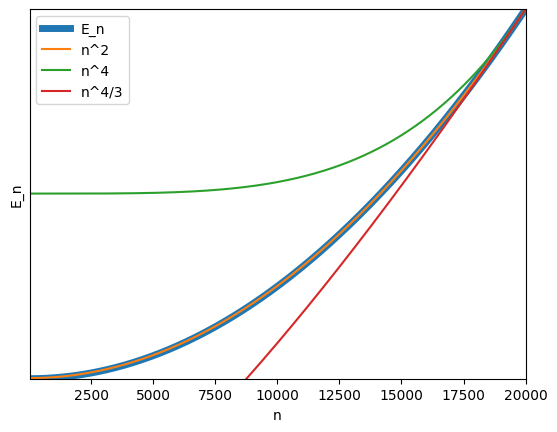
\includegraphics[keepaspectratio, scale=1.0]{temp/fig1.png}
    \caption{\eqref{semiclas_cond}の数値解析の結果}
    \label{py}
  \end{figure}

\end{itemize}

\clearpage
\prb{2}{統計力学}
\begin{enumerate}
  \item 
  可能な配置は
  \begin{equation}
    (\bm{S}_1,\bm{S}_{2})
    =
    (\bm{x},\bm{x})
    \ ,\ \ 
    (\bm{y},\bm{x})
    \ ,\ \ 
    (\bm{x},\bm{y})
    \ ,\ \ 
    (\bm{y},\bm{y})
  \end{equation}
  なので,エネルギーは同じベクトルのときに$-J$,違うベクトルなら$0$となる.また,分配関数は
  \begin{equation}
    Z_{2}
    =
    2+2e^{+J\beta}
  \end{equation}
  である.

  \item 
  $L=3$のときは,
  \begin{equation}
    (\bm{S}_1,\bm{S}_{2},\bm{S}_{3})
    =
    (\bm{x},\bm{x},\bm{x})
    ,
    (\bm{x},\bm{x},\bm{y})
    ,
    (\bm{x},\bm{y},\bm{x})
    ,
    (\bm{y},\bm{x},\bm{x})
    ,
    (\bm{y},\bm{y},\bm{x})
    ,
    (\bm{y},\bm{x},\bm{y})
    ,
    (\bm{x},\bm{y},\bm{y})
    ,
    (\bm{y},\bm{y},\bm{y})
  \end{equation}
  の8通りが可能.それぞれのエネルギーは
  \begin{equation}
    -2J
    \ ,\ 
    -J
    \ ,\ 
    0
    \ ,\ 
    -J
    \ ,\ 
    -J
    \ ,\ 
    0
    \ ,\ 
    -J
    \ ,\ 
    -2J
    \ ,\ 
  \end{equation}
  であり,分配関数は
  \begin{equation}
    Z_{3}
    =
    2+4e^{+\beta J}+2e^{+2\beta J}
  \end{equation}
  である.

  \item 
  分配関数は
  \begin{equation}
    Z_{L}
    =
    \sum_{(\bm{S}_{1},\cdots,\bm{S}_{L-1},\bm{S}_{L})}
    \exp\left[ \beta J \sum_{i=1}^{L-1}\bm{S}_{i}\cdot\bm{S}_{i+1} \right]
  \end{equation}
  である.$\bm{S}_{L}$だけ,別で考えれば
  \begin{equation}
    \sum_{(\bm{S}_{1},\cdots,\bm{S}_{L-1},\bm{S}_{L})}
    \exp\left[ \beta J \sum_{i=1}^{L-1}\bm{S}_{i}\cdot\bm{S}_{i+1} \right]
    =
    \sum_{(\bm{S}_{L-1},\bm{S}_{L})} e^{\beta J\bm{S}_{L-1}\cdot\bm{S}_{L}}
    \sum_{(\bm{S}_{1},\cdots,\bm{S}_{L-1})}
    \exp\left[ \beta J \sum_{i=1}^{L-2}\bm{S}_{i}\cdot\bm{S}_{i+1} \right]
  \end{equation}
  なので,
  \begin{equation}
    Z_{L}
    =
    \sum_{(\bm{S}_{L-1},\bm{S}_{L})} e^{\beta J\bm{S}_{L-1}\cdot\bm{S}_{L}}Z_{L-1}
  \end{equation}
  である\footnote{$L=3$のときをチェックしてみると,ちゃんと成り立ってます.}.

  \item 
  前問から,漸化式は
  \begin{equation}
    \frac{Z_{L-1}}{Z_{L}}
    =
    2(1+e^{\beta J})
  \end{equation}
  である.よって,
  \begin{equation}
    Z_{L}
    =
    2^{L-2}(1+e^{\beta J})^{L-2}Z_{2}
    =
    2^{L-1}(1+e^{\beta J})^{L-1}
    \label{part}
  \end{equation}
  なので,
  \begin{equation}
    F_{L}
    =
    -\frac{1}{\beta}\log Z_{L}
    =
    -\frac{L-1}{\beta}\log 2(1+e^{\beta J})
  \end{equation}
  である.

  \item 
  \eqref{part}より
  \begin{equation}
    u(\beta)
    =
    -\frac{1}{L}\pdv{}{\beta}\log Z_{L}
    =
    -\left( 1-\frac{1}{L} \right)
    \frac{Je^{\beta J}}{1+e^{\beta J}}
    \sim
    -\frac{Je^{\beta J}}{1+e^{\beta J}}
  \end{equation}
  である.低温極限$\beta\gg 1$のときは
  \begin{equation}
    u(\beta)
    \sim
    -J
  \end{equation}
  より,1つのスピン当たりのエネルギーが$J$ということは,スピンの向きがそろっていることを表している.一方で,高温極限$\beta\ll 1$のときは
  \begin{equation}
    u(\beta)
    \sim
    -\frac{J}{2}
  \end{equation}
  より,スピンが無秩序なことを意味している.

  \item 
  $P_{L}(\hat{x},\hat{x})$は
  \begin{equation}    
    P_{L}(\hat{x},\hat{x})
    =    
    P_{L-1}(\hat{x},\hat{x})Q(\hat{x},\hat{x})
    +
    P_{L-1}(\hat{x},\hat{y})Q(\hat{y},\hat{x})
  \end{equation}
  となっている.$L-1$の粒子が$\hat{x}$のとき,$L$の粒子が$\hat{x}$である確率は
  \begin{equation}
    Q(\hat{x},\hat{x})
    =
    \frac{2e^{\beta J}Z_{L-1}}{Z_{L}}
    =
    \frac{e^{\beta J}}{1+e^{\beta J}}
  \end{equation}
  である.同様にして
  \begin{equation}
    Q(\hat{y},\hat{x})
    =    
    \frac{1}{1+e^{\beta J}}
  \end{equation}
  である.このように考えていけば,
  \begin{equation}
    \begin{pmatrix}
      Q(\hat{x},\hat{x}) & Q(\hat{x},\hat{y}) \\
      Q(\hat{y},\hat{x}) & Q(\hat{y},\hat{y})
    \end{pmatrix}
    =
    \frac{1}{1+e^{\beta J}}
    \begin{pmatrix}
      e^{\beta J} & 1 \\
      1 & e^{\beta J}
    \end{pmatrix}
  \end{equation}
  である\footnote{確率の和がちゃんと1になっています.}.

  \item 
  式(2)の右辺を計算すれば
  \begin{equation}
    \begin{pmatrix}
        P_{L}(\hat{x},\hat{x}) & P_{L}(\hat{x},\hat{y}) \\
        P_{L}(\hat{y},\hat{x}) & P_{L}(\hat{y},\hat{y})
    \end{pmatrix}
    =
    \frac{1}{1+e^{\beta J}}
    \begin{pmatrix}
      P_{L-1}(\hat{x},\hat{x}) & P_{L-1}(\hat{x},\hat{y}) \\
      P_{L-1}(\hat{y},\hat{x}) & P_{L-1}(\hat{y},\hat{y})
    \end{pmatrix}
    \begin{pmatrix}
      e^{\beta J} & 1 \\
      1 & e^{\beta J}
    \end{pmatrix}
  \end{equation}
  である.これが漸化式になっているので
  \begin{equation}
    \begin{pmatrix}
      P_{L}(\hat{x},\hat{x}) & P_{L}(\hat{x},\hat{y}) \\
      P_{L}(\hat{y},\hat{x}) & P_{L}(\hat{y},\hat{y})
    \end{pmatrix}
    =
    \frac{1}{(1+e^{\beta J})^{L-2}}
    \begin{pmatrix}
      P_{2}(\hat{x},\hat{x}) & P_{2}(\hat{x},\hat{y}) \\
      P_{2}(\hat{y},\hat{x}) & P_{2}(\hat{y},\hat{y})
    \end{pmatrix}    
    \begin{pmatrix}
      e^{\beta J} & 1 \\
      1 & e^{\beta J}
    \end{pmatrix}^{L-2}
  \end{equation}
  となる.$P_{2}$を計算すれば
  \begin{equation}
    \begin{pmatrix}
      P_{2}(\hat{x},\hat{x}) & P_{2}(\hat{x},\hat{y}) \\
      P_{2}(\hat{y},\hat{x}) & P_{2}(\hat{y},\hat{y})
    \end{pmatrix}    
    =
    \frac{1}{2(1+e^{\beta J})}
    \begin{pmatrix}
      e^{\beta J} & 1 \\
      1 & e^{\beta J}
    \end{pmatrix}
  \end{equation}
  なので\footnote{$Z_{2}$はすでにもとめてあるので,それぞれの状態の$e^{-\beta E}$をもとめて$Z_{2}$で割るだけです.},
  \begin{equation}
    \begin{pmatrix}
      P_{L}(\hat{x},\hat{x}) & P_{L}(\hat{x},\hat{y}) \\
      P_{L}(\hat{y},\hat{x}) & P_{L}(\hat{y},\hat{y})
    \end{pmatrix}
    =
    \frac{1}{2(1+e^{\beta J})^{L-1}}
    \begin{pmatrix}
      e^{\beta J} & 1 \\
      1 & e^{\beta J}
    \end{pmatrix}^{L-1}
    \label{matrixform}
  \end{equation}
  である.よって
  \begin{equation}
    \ev*{\bm{S}_{1}\cdot\bm{S}_{L}}
    =
    P_{L}(\hat{x},\hat{x})
    +
    P_{L}(\hat{y},\hat{y})
  \end{equation}
  なので,\eqref{matrixform}の右辺を求めるだけでよい.行列
  \begin{equation}    
    \begin{pmatrix}
      e^{\beta J} & 1 \\
      1 & e^{\beta J}
    \end{pmatrix}
  \end{equation}
  の固有値と固有ベクトルはそれぞれ
  \begin{equation}
    \begin{dcases}
      \text{固有値}\ \ 
      e^{\beta J}-1
      &:
      \text{固有ベクトル}\ \ 
      \bm{v}_{1}
      =
      \begin{pmatrix}
        1 \\
        -1
      \end{pmatrix}
      \\
      \text{固有値}\ \       
      e^{\beta J}+1
      &:
      \text{固有ベクトル}\ \ 
      \bm{v}_{2}
      =
      \begin{pmatrix}
        1 \\
        1
      \end{pmatrix}
    \end{dcases}
  \end{equation}
  なので,$P=(\bm{v}_{1} \bm{v}_{2})$とおけば,
  \begin{equation}
    P^{-1}
    =
    \frac{1}{2}
    \begin{pmatrix}
      1 & -1 \\
      1 & 1
    \end{pmatrix}
  \end{equation}
  であり,
  \begin{equation}
    \begin{pmatrix}
      e^{\beta J}-1 & 0 \\
      0 & e^{\beta J}+1
    \end{pmatrix}
    =
    P^{-1}
    \begin{pmatrix}
      e^{\beta J} & 1 \\
      1 & e^{\beta J}
    \end{pmatrix}
    P
  \end{equation}
  なので,
  \begin{align*}
    \begin{pmatrix}
      e^{\beta J} & 1 \\
      1 & e^{\beta J}
    \end{pmatrix}^{L-1}
    &=
    P
    \begin{pmatrix}
      (e^{\beta J}-1)^{L-1} & 0 \\
      0 & (e^{\beta J}+1)^{L-1}
    \end{pmatrix}
    P^{-1}
    \nonumber
    \\
    &=
    \frac{1}{2}
    \begin{pmatrix}
      (e^{\beta J}-1)^{L-1}
      +
      (e^{\beta J}+1)^{L-1}
      &
      -(e^{\beta J}-1)^{L-1}
      +
      (e^{\beta J}+1)^{L-1}
      \\
      -(e^{\beta J}-1)^{L-1}
      +
      (e^{\beta J}+1)^{L-1}
      &
      (e^{\beta J}-1)^{L-1}
      +
      (e^{\beta J}+1)^{L-1}
    \end{pmatrix}
  \end{align*}
  である.したがって,\eqref{matrixform}より
  \begin{align}
    &
    \begin{pmatrix}
      P_{L}(\hat{x},\hat{x}) & P_{L}(\hat{x},\hat{y}) \\
      P_{L}(\hat{y},\hat{x}) & P_{L}(\hat{y},\hat{y})
    \end{pmatrix}
    \nonumber
    \\
    &\hspace{1cm}
    =
    \frac{1}{4(1+e^{\beta J})^{L-1}}
    \begin{pmatrix}
      (e^{\beta J}-1)^{L-1}
      +
      (e^{\beta J}+1)^{L-1}
      &
      -(e^{\beta J}-1)^{L-1}
      +
      (e^{\beta J}+1)^{L-1}
      \\
      -(e^{\beta J}-1)^{L-1}
      +
      (e^{\beta J}+1)^{L-1}
      &
      (e^{\beta J}-1)^{L-1}
      +
      (e^{\beta J}+1)^{L-1}
    \end{pmatrix}
  \end{align}
  である.これより
  \begin{equation}
    \ev*{\bm{S}_{1}\cdot\bm{S}_{L}}
    =
    \frac{
    (e^{\beta J}-1)^{L-1}
    +
    (e^{\beta J}+1)^{L-1}}{(1+e^{\beta J})^{L-1}}
    =
    1
    +
    \tanh^{L-1}\left( \frac{\beta J}{2} \right)
  \end{equation}
  である\footnote{よくある計算ではありますが
  \begin{equation}
    \frac{e^{\beta J}-1}{e^{\beta J}+1}
    =
    \frac{e^{\beta J/2}-e^{-\beta J/2}}{e^{\beta J/2}+e^{-\beta J/2}}
    =
    \tanh\left( \frac{\beta J}{2} \right)
  \end{equation}
  です.}.高温極限$\beta\ll 1$では
  \begin{equation}
    \tanh^{L-1}\left( \frac{\beta J}{2} \right)
    =
    \exp\left[ (L-1)\log\tanh\left( \frac{\beta J}{2} \right)  \right]
    \sim
    \exp\left[ -(L-1)\log\frac{2}{\beta J} \right]
  \end{equation}
  なので\footnote{$\tanh x$は
  \begin{equation}
    \begin{dcases}
      \tanh x
      &\sim
      1-e^{-x}
      \ \ \ 
      (x\gg 1)
      \\
      \tanh x
      &\sim
      x
      \hspace{1.2cm}
      (x\ll 1)
    \end{dcases}
  \end{equation}
  です.$x\gg 1$のときのは,グラフを思い出せばなんとなくわかると思います.},
  \begin{equation}
    \ev*{\bm{S}_{1}\cdot\bm{S}_{L}}
    \sim
    1
    +    
    \exp\left[ -(L-1)\log\frac{2}{\beta J} \right]
  \end{equation}
  より,$\xi$は
  \begin{equation}
    \xi
    =
    \frac{1}{\log\frac{2}{\beta J}}
  \end{equation}
  である.一方,低温極限$\beta\gg 1$では
  \begin{equation}
    \tanh^{L-1}\left( \frac{\beta J}{2} \right)
    =
    \exp\left[ (L-1)\log\tanh\left( \frac{\beta J}{2} \right)  \right]
    \sim
    \exp\left[ (L-1)\log\left( 1-\exp\left[ -\frac{\beta J}{2} \right] \right)  \right]
  \end{equation}
  なので,
  \begin{equation}
    \xi
    =
    -
    \frac{1}{\log\left( 1-e^{-\beta J/2} \right)}
    \sim
    e^{\beta J}
  \end{equation}
  である\footnote{$x\ll1$なら,$\log(1+x)\sim x$でした.}.
\end{enumerate}


\clearpage
\prb{3}{力学}
\begin{enumerate}
  \item 
  オイラー・ラグランジュ方程式を解けば
  \begin{equation}
    \left\{
    \begin{alignedat}{1}
      r &:\ 
      \mu\ddot{r}
      -
      \mu r \dot{\varphi}^{2}
      +
      \frac{G\mu M}{r^2}
      =
      0
      \\
      \varphi &:\ 
      2\mu r\dot{r}\dot{\varphi}+\mu r^2 \ddot{\varphi}
      =
      0
    \end{alignedat}  
    \right.
    \label{EOM}
  \end{equation}
  である.

  \item 
  $\varphi$に共役な運動量は
  \begin{equation}
    J
    =
    \pdv{\mathcal{L}}{\dot{\varphi}}
    =
    \mu r^2 \dot{\varphi}
  \end{equation}
  である.また,$r$に共役な運動量を$J_{r}$とすると
  \begin{equation}
    J_{r}
    =
    \pdv{\mathcal{L}}{\dot{r}}
    =
    \mu \dot{r}
  \end{equation}
  なので,エネルギーは,ルジャンドル変換から
  \begin{equation}
    E
    =
    \dot{r} J_{r}
    +
    \dot{\varphi} J
    -
    \mathcal{L}
    =
    \frac{1}{2}\mu\dot{r}^2
    +
    \frac{1}{2}\mu r^2\dot{\varphi}^2
    -
    \frac{G\mu M}{r}
  \end{equation}
  である.

  \item 
  \eqref{EOM}の第2式より
  \begin{equation}
    \dot{J}
    =
    0
  \end{equation}
  なので,$J$は定数.同様にして
  \begin{align*}
    \dot{E}
    &=
    \dv{}{t}\left[  
      \frac{1}{2}\mu\dot{r}^2
      +
      \frac{1}{2}\mu r^2\dot{\varphi}^2
      -
      \frac{G\mu M}{r}
    \right]
    \nonumber
    \\
    &=
    \dot{\varphi}(2\mu r\dot{r}\dot{\varphi}+\mu r^2\ddot{\varphi})
    +
    \dot{r}\left(  
      \mu\ddot{r}-\mu r\dot{\varphi}^2+\frac{G\mu M}{r^2}
    \right)
    \nonumber
    \\
    &=
    0
  \end{align*}
  なので,$E$も定数.

  \item 
  \begin{equation}
    \dv{a}{t}
    =
    -\frac{64 G^3 \mu M^2}{5c^5}\cdot\frac{1}{a^3}
    \ .
    \label{diffeq}
  \end{equation}

  \item 
  式(6)は,形式的に
  \begin{equation}
    P^{5/3} \dd P
    =
    -A(P_{c})^{5/3}\dd t
  \end{equation}
  と書けるので,これを解けば
  \begin{equation}
    \frac{3}{8}P^{8/3}
    =
    -A(P_{c})^{5/3}t + \frac{3}{8}P_{0}^{8/3}
  \end{equation}
  である.$t=\tau_{\text{GW}}$で$P=0$なので
  \begin{equation}
    \tau_{\text{GW}}
    =
    \frac{3P_{0}^{8/3}}{8A}P_{c}^{-5/3}
    \label{tau}
  \end{equation}
  である.

  \item 
  ケプラーの法則を微分すれば
  \begin{equation}
    \dv{a}{t}
    =
    \frac{GMP\dot{P}}{6\pi^2a^2}
    =
    \frac{4^{2/3}G^{1/3}M^{1/3}\dot{P}}{6\pi^{2/3}}\cdot\frac{1}{P^{1/3}}
  \end{equation}
  なので,これを\eqref{diffeq}に代入すれば,
  \begin{equation}
    \dv{P}{t}
    =
    -\frac{64 G^3 \mu M^2}{5c^5}\cdot
    \frac{4\pi^2}{GM}\cdot\frac{1}{P^2}
    \cdot\frac{6\pi^{2/3}P^{1/3}}{4^{2/3}G^{1/3}M^{1/3}}
    =
    -\frac{1536\pi^{8/3}}{5\times 4^{2/3}}\left(  
      \frac{GM^{2/5}c^{-3}\mu^{3/5}}{P}
    \right)^{5/3}
  \end{equation}
  である.$\alpha,\beta,\gamma,A$はこれから決まる\footnote{次元ですが
  \begin{equation}
    G=[M]^{-1}[L]^{3}[T]^{-2}
  \end{equation}
  なので
  \begin{equation}
    GM^{2/5}c^{-3}\mu^{3/5}
    =
    [M]^{-1}[L]^{3}[T]^{-2}
    \cdot
    [M]^{2/5}
    \cdot
    [L]^{-3}[T]^{3}
    \cdot
    [M]^{3/5}
    =
    [T]
  \end{equation}
  でちゃんと時間になってます.
  }\footnote{$A$の値はおおよそ2581となっています.}.

  \item 
  \eqref{tau}より
  \begin{equation}
    P_{c}
    =
    \left( \frac{3}{8A\tau_{\text{GW}}} \right)^{3/5}P_{0}^{8/5}
  \end{equation}
  であり,一方で
  \begin{equation}
    P_{c}
    =
    \frac{GM^{2/5}\mu^{3/5}}{c^3}    
    =
    \frac{Gm}{2^{1/5} c^3}
  \end{equation}
  である.したがって
  \begin{align}
    \frac{m}{M_{\odot}}
    &=
    \frac{2^{1/5}c^3}{GM_{\odot}}\left( \frac{3P_{0}}{8A\tau_{\text{GW}}} \right)^{3/5}P_{0}
    \nonumber
    \\
    &\sim
    10^{5}
    \cdot
    2
    \cdot
    1.1
    \cdot
    \left( \frac{3\times0.06}{8\cdot2500\cdot0.15} \right)^{3/5}
    \cdot
    0.06
    \nonumber
    \\
    &\sim
    38.28
  \end{align}
  である\footnote{3/5乗のところが少し難しいかもしれませんが
    \begin{equation}
      \left( \frac{3\times0.06}{8\cdot2500\cdot0.15} \right)^{3/5}
      =
      \left( \frac{6}{10^5} \right)^{3/5}
      =
      6^{3/5}\times10^{3}
    \end{equation}
    でいけます.
  }\footnote{\href{https://www.ligo.org/science/Publication-GW150914/science-summary-japanese.pdf}{この記事}によると,GW150914は太陽質量のおよそ30倍の天体の合体らしいです.}.

  \item 
  エネルギー
  \begin{equation}
    E
    =
    -\frac{G\mu M}{2a}
    =
    -\frac{Gm^2}{2a}
  \end{equation}
  の差が,$mc^2$の$1/10$だと近似しているので
  \begin{equation}
    -\frac{Gm^2}{2a_{0}}
    +\frac{Gm^2}{2a_{\min}}
    \sim
    \frac{1}{10}mc^2
  \end{equation}
  である.ここで,$a_{0}\gg a_{\min}$より$a_{0}-a_{\min}\sim a_{0}$と近似できるとすれば
  \begin{equation}
    \frac{1}{a_{0}}-\frac{1}{a_{\min}}
    =
    \frac{a_{\min}-a_{0}}{a_{\min}a_{0}}
    \sim
    -\frac{a_{0}}{a_{\min}a_{0}}
    =
    -\frac{1}{a_{\min}}
  \end{equation}
  となるので,
  \begin{equation}
    5Gm
    =
    a_{\min}c^2
  \end{equation}
  である.
\end{enumerate}

\subsection*{補足}

\begin{itemize}
  \item 
  この系の運動は
  \begin{equation}
    \bm{r}_{1}
    =
    \frac{m_{2}}{m_{1}+m_{2}}\bm{r}
    \ ,\ \ 
    \bm{r}_{2}
    =
    \frac{m_{1}}{m_{1}+m_{2}}\bm{r}
    \ ,\ \ 
    \bm{r}
    \coloneqq
    \bm{r}_{2}-\bm{r}_{1}
  \end{equation}
  を用いて書けます.ここで,ポテンシャルの偏りは次の4重極モーメントテンソル
  \begin{equation}
    D_{\alpha\beta}
    =
    J_{\gamma\gamma}\delta_{\alpha\beta}
    -
    3J_{\alpha\beta}
  \end{equation}
  を計算してやると
  \begin{equation}
    \begin{alignedat}{1}  
      D_{xx}
      &=
      \mu r^2(3\cos^2\varphi -1)
      \\
      D_{yy}
      &=
      \mu r^2(\sin^2\varphi-1)
      \\
      D_{xy}
      &=
      3\mu r^2\cos\varphi\sin\varphi
      \\
      D_{zz}
      &=
      -\mu r^2
    \end{alignedat}
  \end{equation}
  となります\footnote{
    ここで,$J_{\alpha\beta}$は慣性モーメントテンソルで,今は
    \begin{equation}
      J_{xx}
      =
      \mu r^2(1-\cos^2\varphi)
      \ ,\  
      J_{yy}
      =
      \mu r^2(1-\sin^2\varphi)
      \ ,\  
      J_{xy}
      =
      -\mu r^2\cos\varphi\sin\varphi
      \ , \ 
      J_{zz}
      =
      \mu r^2
    \end{equation}
    です.
  }.これをもとめてゴニョニョ計算すると
  \begin{equation}
    I
    =
    -\dv{E}{t}
    =
    \frac{32k^4\mu^2M^3}{5c^5r^5}
  \end{equation}
  となり,これが古典力学で近似したエネルギー放射率となっています.

  \item 
  ちなみに,ランダウ・リフシッツ『場の古典論』の演習問題には本問題で省かれているところが載っています.

\end{itemize}



\clearpage
\prb{6}{電磁気学}
\begin{enumerate}
  \item 
  式(1)を$x$で微分して式(2)を代入すれば
  \begin{equation}
    \pdv[2]{I}{x}
    =
    CL
    \pdv[2]{I}{t}
  \end{equation}
  なので,
  \begin{equation}
    v
    =
    \frac{1}{\sqrt{CL}}
  \end{equation}
  である\footnote{
    波動方程式で,どっちの係数が速度なのかを忘れたら,まずは次元をチェックするのが早いです.
  }.

  \item 
  $\lambda=v/f$より
  \begin{equation}
    \lambda
    =
    \frac{1}{f}\cdot\frac{1}{\sqrt{\varepsilon\mu_{0}}}
  \end{equation}
  だが,$\varepsilon=\varepsilon_{r}\varepsilon_{0}$に気をつければ
  \begin{equation}
    \frac{1}{\sqrt{\varepsilon\mu_{0}}}
    =
    \frac{1}{\sqrt{\varepsilon_{r}}}\cdot\frac{1}{\sqrt{\varepsilon_{0}\varepsilon_{0}}}
    =
    \frac{c}{\sqrt{\varepsilon_{r}}}
  \end{equation}
  なので,
  \begin{equation}
    \lambda
    =
    \frac{c}{f\sqrt{\varepsilon_{r}}}
    \sim
    \frac{3.0\times10^8}{500\times10^{6}\times\sqrt{2.2}}
    \sim
    0.405 \text{m}
  \end{equation}
  である.

  \item 
  $V=Z_{0}I$を微分方程式(1),(2)に代入すると
  \begin{equation}
    \left\{
    \begin{alignedat}{1}
      \pdv{I}{x}&=-CZ_{0}\pdv{I}{t}
      \\
      \pdv{I}{x}&=-\frac{L}{Z_{0}}\pdv{I}{t}
    \end{alignedat}
    \right.
  \end{equation}
  なので,係数から
  \begin{equation}
    Z_{0}
    =
    \sqrt{\frac{L}{C}}
  \end{equation}
  である.これに設問2.の条件をいれれば
  \begin{equation}
    Z_{0}
    =
    \frac{\log(b/a)}{2\pi\sqrt{\varepsilon_{r}}}\sqrt{\frac{\mu_{0}}{\varepsilon_{0}}}
    =
    \frac{\mu_{0}c\log(b/a)}{2\pi\sqrt{\varepsilon_{r}}}
  \end{equation}
  である.よって,これを計算すれば
  \begin{equation}
    Z_{0}
    \sim
    \frac{4\times3.14\times10^{-7}\times3\times10^{8}\times1.8}{2\times3.14\times\sqrt{2.2}}
    \sim
    72.8\ 
    \Omega
  \end{equation}
  である\footnote{$V=Z_{0}I$から,単位はオームでいいでしょう.}.

  \item 
  終端で直ちにパルス波が反射されると考えると,到達した瞬間の終端の電圧は$V_{1}+V_{2}$である.一方で,抵抗器を流れる電流は$I_{1}-I_{2}$である.ただし,$I_{1},I_{2}$は
  \begin{equation}
    V_{1}=Z_{0}I_{1}
    \ ,\ \ 
    V_{2}=Z_{0}I_{2}
    \label{current}
  \end{equation}
  を満たす電流である.よって,抵抗器の回路に対するオームの法則から
  \begin{equation}
    V_{1}+V_{2}
    =
    r(I_{1}-I_{2})
  \end{equation}
  が成立し,この関係式に\eqref{current}を代入すれば
  \begin{equation}
    V_{2}
    =
    \frac{r-Z_{0}}{r+Z_{0}}
    V_{1}
  \end{equation}
  である\footnote{$r=Z_{0}$で$V_{2}=0$なのでOK.}.

  \item 
  式(4)を$x$で微分して式(1)を代入すれば
  \begin{equation}
    \pdv[2]{V}{x}
    =
    LC\pdv[2]{V}{t}
    +
    RC\pdv{V}{t}
  \end{equation}
  である.特解として$V=\tilde{V}(x)e^{-i\omega t}$を考えると,
  \begin{equation}
    \pdv[2]{\tilde{V}}{x}
    =
    -C\omega(L\omega+iR)\tilde{V}
  \end{equation}
  である.$\Omega\coloneqq\sqrt{C\omega(L\omega+iR)}$としておくと,これの解は
  \begin{equation}
    \tilde{V}(x)
    =
    Ae^{i\Omega x}
    +
    Be^{-i\Omega x}
    \label{gen_sol}
  \end{equation}
  と書ける.ここで,$\Omega$は
  \begin{equation}
    \Omega
    =
    \omega\sqrt{LC}\sqrt{1+i\frac{R}{L\omega}}
    \sim
    \omega\sqrt{LC}\left( 1+i\frac{R}{2L\omega} \right)
  \end{equation}
  と書けるとすれば,\eqref{gen_sol}のうち,採用できるのは$A=V_{1},B=0$のみであり\footnote{もし,$B\neq 0$なら,$x\rightarrow\infty$に対して$\tilde{V}(x)\rightarrow\infty$となるような解が出てきてしまいます.また,$B=0$なら$x=0$の初期条件から$A=V_{1}$です.},
  \begin{equation}
    \tilde{V}(x)
    =
    V_{1}\exp\left[ -\frac{R}{2}\sqrt{\frac{C}{L}}x \right]e^{i\omega\sqrt{LC}x}
  \end{equation}
  である.よって,$V_{2}=|\tilde{V}(d)|$なので
  \begin{equation}
    V_{2}
    =
    V_{1}\exp\left[ -\frac{Rd}{2}\sqrt{\frac{C}{L}} \right]
    \ \text{or}\ 
    V_{1}e^{-Rd/2Z_{0}}
  \end{equation}
  である.

  \item 
  セットアップは
  \begin{equation}
    \left\{  
      \begin{alignedat}{1}
        \nabla\times\bm{B}
        &=
        \mu\bm{j}
        \\
        \nabla\times\bm{E}+\pdv{\bm{B}}{t}&=0
        \\
        \bm{j}&=\sigma\bm{E}
      \end{alignedat}
    \right.
  \end{equation}
  である.ただし,電場$\bm{E}$の時間微分は,電場の時間変動は非常に小さいとして無視した.第1式を時間微分して,$\nabla\times(\nabla\times\bm{A})=\nabla(\nabla\cdot\bm{A})-\nabla^2$を用いれば
  \begin{equation}
    \nabla^2\bm{E}
    =
    \mu\pdv{\bm{j}}{t}
  \end{equation}
  である.ただし,$\nabla\cdot\bm{E}=0$とした.これはオームの法則より,
  \begin{equation}
    \frac{1}{\sigma}\nabla^2\bm{j}
    -
    \mu\pdv{\bm{j}}{t}
    =
    0
  \end{equation}
  である.これは一般的な話なので,軸方向に限って言えば
  \begin{equation}
    \pdv[2]{j}{r}
    +
    \frac{1}{r}\pdv{j}{r}
    -
    \mu\sigma\pdv{j}{t}
    =
    0
  \end{equation}
  が成立する\footnote{
    ただし,
    \begin{equation}
      \nabla^2
      =
      \frac{1}{r}\pdv{}{r}\left( r\pdv{}{r} \right)
      +
      \frac{1}{r^2}\pdv[2]{}{\varepsilon}
      +
      \pdv[2]{}{z}
    \end{equation}
    を用いた.
  }.これに$j(r,t)=J(r)e^{-i\omega t}$を代入すれば,
  \begin{equation}
    \pdv[2]{J(r)}{r}
    +
    \frac{1}{r}\pdv{J(r)}{r}
    -
    i\omega\mu\sigma J(r)
    =
    0
    \label{PDE}
  \end{equation}
  である.今回は,$r\sim a$の付近で
  \begin{equation}
    J(r)
    =
    |J(a)|e^{(r-a)/\delta}\cdot e^{iA}
  \end{equation}
  と近似できるとすれば,\eqref{PDE}に代入すれば
  \begin{equation}
    \frac{1}{\delta^2}
    +
    \frac{1}{r}\cdot\frac{1}{\delta}
    -
    e^{i\pi/2}\omega\mu\sigma
    =
    0
  \end{equation}
  である.ここで,今考えているのは$r\sim a\gg \delta$付近の話であり,$1/r$を含む項はとても小さいので無視することができる.よって
  \begin{equation}
    \delta
    =
    \Re
    \left[  
      e^{-i\pi/4}\sqrt{\frac{1}{\omega\mu\sigma}}
    \right]      
    =
    \sqrt{\frac{2}{\omega\mu\sigma}}
  \end{equation}
  が表皮の深さである.

\end{enumerate}

\subsection*{補足}

\begin{itemize}
  \item 
  設問6.は誘導に従いましたが,一般には\eqref{PDE}はベッセル関数で書けます.ベッセルの微分方程式は
  \begin{equation}
    \dv[2]{u}{z}
    +
    \frac{1}{u}\dv{u}{z}
    +
    \left( 1-\frac{n^2}{z^2} \right)u
    =
    0
  \end{equation}
  であり,この解は,次のベッセル関数
  \begin{equation}
    J_{n}(z)
    =
    \sum_{m=0}^{\infty}\frac{(-1)^{m}}{m!(n+m)!}\left( \frac{z}{2} \right)^{n+2m}
  \end{equation}
  で与えられます\footnote{
    代入すればわかります.
  }.\eqref{EOM}を$k^2\coloneqq -i\omega\mu\sigma$として,$z=kr$と変数変換すれば
  \begin{equation}
    \pdv[2]{\tilde{J}(z)}{z}
    +
    \frac{1}{z}\pdv{\tilde{J}(z)}{z}
    +
    \tilde{J}(z)
    =
    0
  \end{equation}
  なので,これは$n=0$のベッセルの微分方程式です.よって,$J$は
  \begin{equation}
    J(r)
    \propto
    J_{0}(kr)
  \end{equation}
  になります.

\end{itemize}


\end{document}
